\documentclass[11pt]{article}

\usepackage[T1]{fontenc}
\usepackage[utf8]{inputenc}
\usepackage{charter}
\usepackage[scaled=0.9]{helvet}
\usepackage{courier}
\usepackage[margin=1in]{geometry}
\usepackage{microtype}
\usepackage{amsmath,amssymb}
\usepackage{booktabs}
\usepackage{tabularx}
\usepackage{longtable}
\usepackage{array}
\usepackage{enumitem}
\usepackage[dvipsnames]{xcolor}
\usepackage{tikz}
\usetikzlibrary{arrows.meta,positioning,calc,shapes.geometric,fit}
\usepackage{fancyvrb}
\usepackage[hidelinks]{hyperref}
\usepackage{titlesec}
\usepackage{caption}

\setlist{itemsep=2pt,topsep=4pt}
\setlength{\parskip}{4pt}
\setlength{\parindent}{0pt}
\setlength{\emergencystretch}{2.5em}
\renewcommand{\arraystretch}{1.18}
\captionsetup{font=small,labelfont=bf}

\usepackage{url}
\urlstyle{tt}
\makeatletter
\g@addto@macro{\UrlBreaks}{\do\_\do\:\do\-\do\,\do\/}
\makeatother
\newcommand{\code}{\path}
\newcolumntype{L}{>{\raggedright\arraybackslash}X}
\newcolumntype{P}[1]{>{\raggedright\arraybackslash}p{#1}}
\newcolumntype{R}[1]{>{\raggedleft\arraybackslash}p{#1}}

\definecolor{accent}{RGB}{176,58,46}
\definecolor{soft}{RGB}{245,240,236}
\definecolor{ok}{RGB}{39,110,72}

\newenvironment{keypoint}{\begin{center}
\begin{tikzpicture}\node[draw=accent,fill=soft,rounded corners=2pt,inner sep=8pt,text width=0.92\linewidth]\bgroup}{\egroup;\end{tikzpicture}\end{center}}

\title{\textbf{Breaking the Validator Stall Loop}\\[4pt]
\large Cost-accounted order-then-execute, built on the cost-accounting papers:\\ analysis, design, throughput model, and the path to a working branch}
\author{F1R3FLY.io --- design document, revision 5}
\date{October 29, 2026}

\begin{document}
\maketitle

\begin{center}
\small
\begin{tabular}{@{}lP{10.6cm}@{}}
\toprule
Repository & \code{F1R3FLY-io/f1r3node-rust} \\
Code basis & \code{dev} at \code{252a86d1d} (Oct 28, 2026); Track~A on \code{fix/finality-stall-track-a}, \code{fix/finalizer-forward-progress} and \code{fix/stall-track-a-rest}; \code{integration/cost-accounted-ote-b1d866e45} at \code{d1f3ab5e1}, which carries Track~A and the B4 work through patch 0035 \\
Design basis & The cost-accounting papers in \code{F1R3FLY-io/publications} at \code{37915af} (Oct 28, 2026), read directly (\S\ref{sec:sources}) \\
Revision 5 & Records the answers to Q-14 to Q-17 and the decisions that followed. REV is conserved and minted only at genesis from \code{wallets.txt}. Phlo is a rate, not a token: nothing is minted per deployment and there is no escrow; the gate records a commitment against the wallet. Behaviour beyond the core enters through hooks that default to no-ops, under a multi-signature authority named at genesis. Box-car batching of debits is a node parameter, and a canonical settled form keeps it out of the state root. There is no legacy chain to preserve. Adds the path to a working branch (\S\ref{sec:plan}): current \code{dev}, a reduced Track~A, and three phases, in place of the S1--S7 series. Corrects revision~4, which listed Track~A as delivered on \code{dev}; it is not. \\
Revision 4 & Recorded the agreed relationship between REV and the token stacks. Wallets are disaggregated from the vault: REV lives in located stacks on its owners' channels, and moving REV is a native operation. Phlo is what a COMM spends, minted per deployment at the deployment's stated price. The system is linear: REV changes hands, and is never created or destroyed by computation. Consumed REV moves to the proposer that the block names. Revision~3 treated the vault as permanent and REV payments as a later track; that part is withdrawn. \\
Revision 3 & Rebuilt the cost-accounting design on the papers and added a measured throughput model. The stall analysis, the consensus seam and the finalizer design of revision~2 stand. \\
Method & Code reading, and measurements on a 2-vCPU host (Intel Xeon at 2.1\,GHz, release build). Absolute times are host-specific. The ratios carry the argument. \\
\bottomrule
\end{tabular}
\end{center}

\begin{abstract}
\noindent Validators stall as they come under sustained load. The stall analysis of revisions 1 and~2 stands: a feedback loop through the finality lag, closed by two hard limits, with run-to-completion execution and the merge it forces at its root. This revision builds the cost-accounting half of the design on the papers. Wallets are disaggregated from the vault: each wallet is a stack of REV located on its owner's own channel, so moving REV is a native operation on two channels, with no shared contract on its path. A deployment states a phlo limit and a phlo price. A validator accepts or rejects it on that price. Phlo is the rate at which REV is spent: the gate checks that the wallet covers the overestimate at that price and records a commitment, nothing leaves the wallet, and each COMM moves REV at that price from the wallet to the block's proposer. The system is linear: REV is created once, at genesis, every unit of work happens because REV changes hands, and nothing is burned. The implementation today keeps money in the SystemVault, reads it through Rholang contracts, and settles every deploy through one shared vault contract that burns the charge. Measured on the integration branch, settlement takes 83--94\,\% of block execution, and a one-line deploy spends 1.2\,ms interpreting its term and about 675\,ms on funding and settlement. The throughput model projects a 12--105-fold reduction of per-envelope work on the measured workloads, about 100-fold for REV transfers, and near-linear scaling with cores for envelopes with independent signers. That is two to three orders of magnitude over today's measured 0.44--1.24 envelopes per second for small deploys and transfers, and one to two orders for heavier deploys. The model also identifies where the gains stop: deploys dominated by their own computation, application-level hot channels, the consensus cap of envelopes per block, and multi-core RSpace efficiency, which is not yet measured. The quickest path to a working branch starts from current \code{dev}, adds the part of Track~A that \code{dev} lacks, ports the consensus seam, and builds the native REV layer on it: about five to six and a half engineer-weeks to a mergeable branch with the core of the design.
\end{abstract}

\tableofcontents
\newpage

%======================================================================
\section{Summary}

\textbf{The stall.} Under sustained deploy load the unfinalized region of the DAG grows. Proposal preparation, merging, the deploy lifecycle register and the finality oracle all do work that grows with that region, which slows blocks and finality, which grows the region. Two limits turn the slowdown into a stop: a 15-second finalizer timeout that discards all work, and a merge cap at 256 blocks of floor distance (\S\ref{sec:analysis}). Track~A holds the fixes for the finality half of the loop. It has not reached \code{dev}, which has meanwhile landed its own versions of several of them (\S\ref{sec:plan}).

\textbf{The cause underneath.} Each deploy runs to completion against committed state, so concurrently produced blocks hold divergent post-states, and the node must merge them. The cost-accounting papers remove the reason for the merge: every interaction is gated by a token of the signatures involved, so potential conflicts are visible as shared signatures, and deploys can run at any time.

\textbf{The two central points of the design.}
\begin{enumerate}
\item \textbf{No hot spots.} Wallets are disaggregated from the vault. Each wallet is a stack of REV located on its owner's own channel. A deploy touches only the wallets and stacks that its own signatures name. Two deploys with different signers touch disjoint state and cannot contend. A shared structure on the payment path would put every deploy on one causal chain, and that is what the papers rule out.
\item \textbf{Concurrent deploys, little merge logic.} Acceptance by linear proof is the concurrency control. Competing deploys are competing proof obligations over the same linear hypotheses, and at most one succeeds before any step runs. Independent deploys then run concurrently. The only conflicts left are races on shared data channels, which the runner decides and records.
\end{enumerate}

\textbf{REV and phlo.} REV is the quantity held in wallets. Phlo is what a COMM spends. A deployment states a \code{phloLimit} and a \code{phloPrice}, and a validator accepts or rejects it on that price. Phlo is not minted: it is the rate at which wallet REV is spent per COMM. At acceptance, the gate checks that the wallet covers the overestimate at the deployment's price and records a commitment; nothing moves. Each COMM moves \code{phloPrice} REV from the wallet to the proposer's channel, and at settlement the commitment is released. The system is linear: REV is minted only at genesis, from \code{wallets.txt}, work happens because REV changes hands, REV is never created or destroyed by computation, and the counterparty of every payment is a name in the term that the block fixes (\S\ref{sec:linear}).

\textbf{Where the implementation stands.} The consensus seam is largely in place: order-then-execute, structural validity, the linearizer, records, attestation, inclusion checks and pruning (patches 0028--0035). The funding path departs from the papers. Money stays in the SystemVault. Each deploy reads vault balances through Rholang (44.5\,ms per read), and after its run one vault contract reserves, validates, apportions, burns the charge, pays a shared fee vault and refunds. That play runs with an unlimited budget and writes about 1{,}000 events into the record. A user REV transfer through the vault costs 81.6\,ms of contract code on its own. Every settlement touches the same vault map, fee vault and cost cursors, so settlements form one causal chain. The measured consequence: settlement is 83--94\,\% of block execution, and the branch executes 0.44--1.24 envelopes per second on the measurement host (\S\ref{sec:measured}).

\textbf{Projected throughput.} Per-envelope work falls 12- to 105-fold on the measured workloads and about 100-fold for REV transfers, and independent envelopes scale with cores. For one-line deploys and transfers the projection is about 160--280 envelopes per second on the 2-vCPU measurement host and 1{,}300--2{,}250 on 16 cores, against 0.44--1.24 today. Where gains are smaller, \S\ref{sec:limits} explains why, item by item.

\begin{keypoint}
\textbf{Decisions (\S\ref{sec:decisions}).} Items 1 to 4 are agreed; item 5 is proposed.
\begin{enumerate}[label=(\arabic*),leftmargin=1.5em]
\item Wallets are located REV stacks on their owners' channels, disaggregated from the vault. Moving REV is native.
\item REV is conserved and minted only at genesis. Phlo is a rate, not a token, and there is no escrow. The shard minimum price is a validity floor; the validator's price is a fixed node price behind a hook.
\item Consumed REV moves to the proposer that the block names. Nothing is burned, and there is no fixed fee apart from phlo.
\item Hooks default to no-ops and change only by a multi-signature of addresses named at genesis. Box-car batching is a node parameter that never changes the state root.
\item The base is current \code{dev} with a reduced Track~A, then the seam and the native REV layer in three phases (\S\ref{sec:plan}).
\end{enumerate}
\end{keypoint}
\section{What revisions 3 to 5 change, and why}\label{sec:changes}

Revision~2 stated in its sources that it ``did not read the papers directly'', and took them as the branch's proposal quoted them. It got the signature-marking argument right: different signatures cannot conflict on funding, and agreement reduces to the race winners of each block and the order of conflicting blocks. It missed what the papers say about money. It does not mention token stacks. It adopted the branch's settlement as a library to port. It kept the vault's contention patch as a requirement (``\code{SystemVault.rho} bucket locks (DR-119): Keep''). It defined the record to include ``settlements, system work'', so the vault's event logs entered consensus.

The work of the week of October 26 traced each of these to a defect:
\begin{itemize}
\item \textbf{Record size.} Records came to about 100\,KB per envelope, 93\,\% logs, and 92\,KB of that was the vault settlement log. A block of more than about 80 envelopes produced a record that no block could carry (patch 0035).
\item \textbf{Unbounded system work.} Settlement runs with \code{Cost::unsafe_max()}, the gate's estimator cannot bound the vault contracts, and system plays never draw on the meter: a test measured 0 phlo under any budget.
\item \textbf{The vault as a hot spot.} A precharge-and-refund design built on the vault measured worse than the code it replaced: 118\,KB per one-source send. That design is withdrawn.
\end{itemize}

Revision~3 started from the papers and measured the gap. It still treated the vault as the permanent custodian of REV, with tokens bought from it at a boundary, and it put REV payments in a later track. Revision~4 corrects that. The papers' abstraction is a disaggregation of wallets from the vault: REV itself lives in located stacks, and every payment is REV changing hands in a linear system. Revision~5 takes the last two steps of that correction. Phlo is not a token at all, so there is nothing to mint and nothing to hold in escrow: it is the rate at which REV in the wallet is spent. And REV itself is minted once, at genesis. With custody, escrow, cursors and the legacy path gone, the implementation no longer needs most of the integration branch, and the quickest path to it starts from current \code{dev}.

Everything in revision~2 that does not depend on the funding path stands: the stall analysis, the consensus seam, the canonical order, records and attestation, the finalizer design, backpressure, Track~A and the hook points.
\section{The stall: analysis}\label{sec:analysis}

This section restates revision~2 in brief. The evidence and line references are unchanged, and Appendix~\ref{app:findings} lists the detailed findings.

\subsection{The core loop}

Under sustained load three quantities grow together: the pending deploy pool, the set of deploys included in blocks but not yet settled, and the unfinalized DAG cone. Each grows with the finality lag $D$, and each carries costs that scale with it (Figure~\ref{fig:loop}).

\begin{figure}[h]
\centering
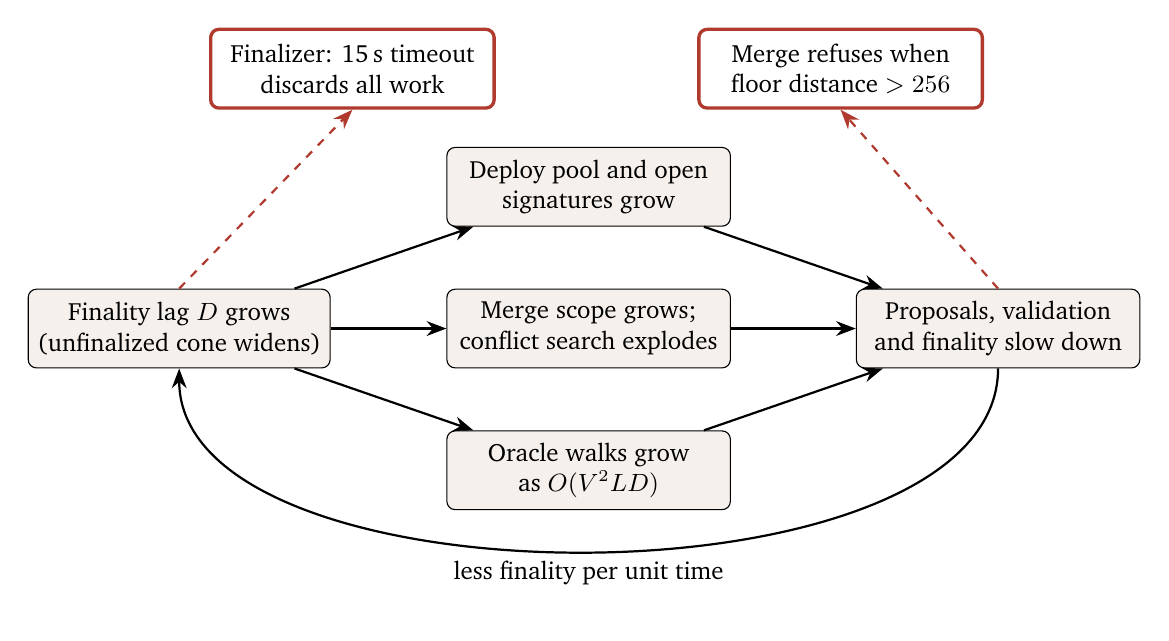
\begin{tikzpicture}[
  box/.style={draw,rounded corners=3pt,fill=soft,align=center,minimum width=3.6cm,minimum height=1.0cm,font=\small},
  trap/.style={draw=accent,very thick,rounded corners=3pt,fill=white,align=center,minimum width=3.6cm,minimum height=1.0cm,font=\small},
  arr/.style={-{Stealth[length=2.5mm]},thick}]
\node[box] (lag) at (0,0) {Finality lag $D$ grows\\(unfinalized cone widens)};
\node[box] (pool) at (5.2,1.8) {Deploy pool and open\\signatures grow};
\node[box] (merge) at (5.2,0) {Merge scope grows;\\conflict search explodes};
\node[box] (fin) at (5.2,-1.8) {Oracle walks grow\\as $O(V^2 L D)$};
\node[box] (slow) at (10.4,0) {Proposals, validation\\and finality slow down};
\draw[arr] (lag) -- (pool);
\draw[arr] (lag) -- (merge);
\draw[arr] (lag) -- (fin);
\draw[arr] (pool) -- (slow);
\draw[arr] (merge) -- (slow);
\draw[arr] (fin) -- (slow);
\draw[arr] (slow.south) .. controls (10.4,-3.6) and (0,-3.6) .. node[below,font=\small]{less finality per unit time} (lag.south);
\node[trap] (t1) at (2.2,3.3) {Finalizer: 15\,s timeout\\discards all work};
\node[trap] (t2) at (8.4,3.3) {Merge refuses when\\floor distance $>256$};
\draw[arr,accent,dashed] (lag.north) -- (t1.south);
\draw[arr,accent,dashed] (slow.north) -- (t2.south);
\end{tikzpicture}
\caption{The feedback loop. Every cost in the middle column grows with the finality lag. The two traps (outlined) turn the slowdown into a stop.}
\label{fig:loop}
\end{figure}

\subsection{Costs that grow with the lag, and the starvation paths}

\begin{itemize}
\item \textbf{Deploy pool.} About $8N$ signature checks per proposal for a pool of $N$, re-read under a lock.
\item \textbf{Lineage walks.} Quadratic in load: open signatures times segment length times deploys per block.
\item \textbf{Rejection-option search.} Exponential in conflicting pairs per group. Vault and PoS channels collapse groups into one, so the vault is a hot spot for the merge as well.
\item \textbf{Hot channels in RSpace.} $O(n)$ per touch and $O(n^2)$ over a run for a channel that accumulates $n$ datums. Replay scans its COMM list with a copy per step, $O(n^2)$ in COMMs (clone audit, finding~0.2).
\item \textbf{Finality walks.} $O(P \cdot V^2 L D)$ warm per block.
\item \textbf{Starvation.} A serial proposer queue, synchronous locks in async code, and CPU-bound consensus work on the async workers that also serve the network.
\end{itemize}

\subsection{Soak evidence}

The branch's proposal records two soaks. In August one merge call averaged 2.16\,s, 92\,\% of it settled-signature probes. In October no single stage separated failing sessions from passing ones, and the binding constraint had moved toward finality and Casper bookkeeping. The production high-phase replay targets recorded in \code{cost_accounting_perf_spec.rs} attribute about 229\,ms per deploy to precharge, 189\,ms to refund and 32\,ms to evaluation. That is, 93\,\% of replay time per deploy is spent moving money through the vault.

%======================================================================
\section{The blueprint: what the papers specify}\label{sec:blueprint}

This section reads the design from the papers. Each point ends with its consequence for the implementation.

\subsection{Signatures are names; token stacks are located terms}

The cost-accounted rho calculus extends names to $x, y ::= \lceil T \rceil \mid s$: signatures are channel names. Token stacks $S ::= () \mid s : S$ are first-class terms. Each layer is a balance cell of one signature. The companion paper refines the stack to a \emph{located} stack $S(I, s : S')$, a stack indexed by the surface $I$ that may draw on it. In rho this is a token stack sitting on a specific channel: only processes holding a matching channel name can consume from it. Unforgeable channels make that a genuine capability.

\emph{Consequence.} A signer's funds for computation are a stack on the signer's own channel in RSpace. They are not a balance in a shared contract.

\subsection{Payment is the communication}

The five rewrite rules are the COMM rule gated by token consumption. For a single signature,
\[
\{\, \mathtt{for}(y \leftarrow x)\,T \mid x!(U) \,\}_s \;\mid\; s : S \;\longrightarrow\; T\{\lceil U\rceil/y\} \;\mid\; S .
\]
The other four rules cover compound signatures and split or combined tokens. Joins follow one schema quantified over partitions, and conservation of authority holds across all of them: a join consumes exactly one receiver authority and one sender authority per channel.

\emph{Consequence.} The reducer charges by popping cells from located stacks. There is no separate settlement step that converts usage into money after the fact.

\subsection{Acceptance by linear proof is the concurrency control}

A deployment is accepted if and only if a linear proof of its resource use exists: for every signature $s$ it names, the supply $\Sigma_s$ meets the demand $\Delta_s$. The check runs before any step executes, and it is linear in the size of the AST. In the papers' words, two deployments competing for the same tokens are ``two proof obligations competing for the same linear hypotheses. At most one can succeed.'' Duplicate and simultaneous arrivals are resolved by the same rule, ``without locks, priority queues, or rollback mechanisms''.

\emph{Consequence.} Admission needs only the stacks of the envelope's own signers. Group decisions, later holds and shared cursors are unnecessary: committing tokens to an accepted deployment removes them from the supply that the next proof sees.

\subsection{Overcharge and refund}

Where control flow is data-dependent, the validator computes a conservative demand $\Delta^{\max}_c$, the maximum over reachable branches, and accepts if $\Sigma_c \ge \Delta^{\max}_c$. Execution consumes only the tokens it forces, and ``the residual $\Delta^{\max}_c - \kappa$ is returned to the client's token stack as part of the deployment's settlement''. The refund is safe because the number of tokens consumed equals the number of forced redexes, which the runtime counts exactly.

\emph{Consequence.} Settlement is a return of unused cells to the client's own stack. It is not a vault transaction.

\subsection{Located purses make the proof local}

Locating stacks decomposes the global resource obligation into one local linear proof per purse. The global proof is the separating conjunction of the local ones (companion paper, ``Local sufficiency composes''). Location also quarantines data-dependence to the surfaces that need a conservative bound.

\emph{Consequence.} The gate checks each signer's stack independently, and independent signers' checks can run concurrently.

\subsection{Chains and antichains: where hot spots come from}

The spacetime paper maps a cost-accounted computation to a measured causal set. Events are COMM firings, the order is enabling, and concurrency is Bernstein independence of footprints: no write-write and no read-write overlap. Two of its results bear directly on throughput:
\begin{itemize}
\item \textbf{Time from the stack.} The firings that draw on a single located stack form a chain, ordered by stack depth. A shared stack, or any shared resource that every deploy writes, serializes every deploy that touches it.
\item \textbf{Space from the surfaces.} Firings that draw on distinct stacks at non-near surfaces are concurrent: they form an antichain.
\item \textbf{Number is volume.} The phlogiston spent equals the number of events, and discrete proper time is the longest chain.
\end{itemize}
With $W$ the total work and $L$ the longest chain, a scheduler on $P$ cores completes the work in at most $W/P + L$ (Brent's bound). Throughput therefore depends on keeping $L$ short: no state that every deploy writes.

\emph{Consequence.} A design meets the papers' throughput promise only if nothing on the payment path is shared across signers. A shared vault map, fee vault or cursor puts every settlement on one chain, and $L$ grows with $W$.

\subsection{Fees, minting, sponsors and multi-signature}

\begin{itemize}
\item \textbf{Fees.} In the worked example, the validator handler takes one token from the client's address $A_c$ and keeps it on its own fee channel $F_v$. The fee lands on a per-validator channel.
\item \textbf{Minting.} Minting is constructing a token stack and sending it on a signature channel. Epoch phlogiston for validators, slush funds and fee-to-stake conversion use the same primitive.
\item \textbf{Funding slots.} A contract creates an unforgeable channel and lets any funder deposit tokens on it. This decouples who authorizes, who pays and what runs. A sponsor funds a new user through a slot.
\item \textbf{Multi-signature.} A compound signature $s_1 \otimes s_2$ needs tokens from every component. Weakening is forbidden, so a compound token must be spent in full or explicitly split.
\end{itemize}

\emph{Consequence.} Sponsors, grants and owners are funding slots and located stacks, not post-run vault debits.

\subsection{Wallets disaggregated from the vault}

The located stack is how value is held, not only how fuel is held. A wallet is a stack of REV located on its owner's channel. The channel is a function of the owner's signature: a public key, an unforgeable name, or a compound signature for a multi-signature wallet. Finding a wallet is therefore a computation, not a lookup in a shared map. Only a term signed by the owner can draw on the stack. Anyone can deposit to it, as anyone can fund a funding slot.

Cells carry amounts. A balance is a count on a cell, not a list of unit cells, so spending splits a cell and receiving adds one. Deposits land as separate datums on the payee's channel and are combined only when the payee spends. Payments to one payee therefore commute: two deposits never conflict, and only spends from one wallet form a chain.

\emph{Consequence.} Moving REV is a COMM on the payer's and payee's channels. It needs no registry lookup, no map walk, no purse split through a shared mint and no settlement afterwards.

\subsection{Linearity: work happens because REV changes hands}\label{sec:linear}

Linear proofs work because the system is linear. Every token is consumed exactly once, and consuming it moves it to someone. Computation never creates or destroys REV. So the destination of consumed REV is not a policy choice: it moves to the party that the term names as the counterparty.

Phlo is not a second currency. It is the rate at which REV in a wallet is spent: each COMM costs one phlo, and one phlo is \code{phloPrice} REV. Nothing is minted per deployment and nothing is held in escrow. The REV stays in the wallet until a COMM spends it.

A minimal example: client $c$ holds $r$ REV in its wallet $W_c$. Its deployment is one COMM, so $\Delta = 1$ phlo, at price $p$. Validator $v$ proposes the block that includes it.

\begin{Verbatim}[fontsize=\footnotesize,frame=single,framesep=6pt]
D  =  { x!(5) | for(y <- x) Nil }_c           -- one COMM, signed by c

block b, sender v, at D's canonical position:

  W_c!(r) | D                                -- c's wallet: r REV

gate:   r >= Delta * p = p                   -- accept; commit p against W_c
                                             -- (bookkeeping, nothing moves)

-> Rule 1, at price p (k = 1):
  { x!(5) | for(y <- x) Nil }_c | W_c!(r)
    ->  Nil | W_c!(r - p) | F_v!(p)          -- the COMM moves p REV from W_c to F_v

-> release the commitment (Delta - k = 0 unspent: nothing to return)

conservation:  (r - p) at W_c  +  p at F_v  =  r
\end{Verbatim}

The recipient is a name in the term, $F_v$, and $v$ is the block's sender. The term is fixed when $v$ proposes the block. Whoever reduces it, the runner or any replaying validator, reaches the same post-state, and appears nowhere in the term. Paying the runner would make executed state depend on who produced the record, not on the ordered blocks. So consumed REV moves to $F_{\mathrm{sender}(b)}$, and running and replaying are the work every validator does as a member of the shard.

Overcharge and refund keep their meaning without an escrow. The gate commits $\Delta^{\max} \times p$ against the wallet, and execution spends $\kappa \times p$. The residual $(\Delta^{\max} - \kappa) \times p$ never left the wallet, so the ``refund'' is the release of the commitment.

\emph{Consequence.} Conservation is an invariant of every block, and of the shard: the sum over wallets and validator channels equals the genesis supply. There is no burn, no fixed fee and no mint after genesis.

\subsection{Internalisation}

The papers give a source-to-source translation of the cost-accounted calculus into pure Rholang~1.1, with splitter and joiner infrastructure. This gives cost-accounted semantics on today's runtime while the native implementation is built. The history-and-cost note adds that such an internalisation is lax: it carries an overhead grade. The native implementation is therefore the throughput path, and the translation is a bridge.

%======================================================================
\section{The gap, measured}\label{sec:measured}

\subsection{How the funding path works today}

The branch already has the papers' mechanism, but the v6 path does not use it:
\begin{itemize}
\item \textbf{Located stacks exist.} The reducer evaluates a token stack term by producing a \code{CostStack} datum on the signature channel of its head cell (\code{reduce.rs}, \code{eval_cost_stack}). The supply module models purse stacks and their inventory (\code{costacc/supply.rs}). Stack pops are accounted natively (\code{accounting/authority.rs}, \code{stack_pops}).
\item \textbf{v6 offers bypass them.} An owner-direct offer funds ``every class of the signer's own principal lane'' from the signer's vault (\code{owner_offer.rs}). The gate's supply ``counts SystemVault balances only'' (\code{gate.rs}). Fresh usage is bought from REV at the signed price on every deploy.
\end{itemize}

\begin{longtable}{@{}P{4.4cm}P{5.2cm}P{5.4cm}@{}}
\toprule
\textbf{Blueprint} & \textbf{Implementation (v6 path)} & \textbf{Measured effect} \\
\midrule
\endhead
Supply is the depth of the signer's located stack. & Supply is read from SystemVault balances through Rholang queries. & 44.5\,ms per balance query. The run phase spends 110--160\,ms beyond interpreting the term. \\
Payment is the COMM popping a cell. & The run is metered natively. The charge is then converted to REV and settled by \code{applyPhloCost}. & 560--600\,ms and about 1{,}000 events per envelope, under \code{Cost::unsafe_max()}. \\
Refund returns $\Delta^{\max} - \kappa$ to the client's stack. & \code{reserveAll}, \code{validateSettlement} and \code{settleReserved} run together after the run. & The reserve-and-refund happens, collapsed into one play after the run. \\
The linear proof is the concurrency control. & Holds that move no funds, plus \code{decide_groups}, \code{LaterHolds}, a held-capacity guard and the DR-28 cursors. & Settlement runs sequentially in block order. \\
Consumed REV moves to the counterparty; the system is linear. & \code{settleReserved} burns the resource charge, leaving it in a purse that nobody can reach. Only the fee moves. & REV is destroyed by computation, which breaks conservation. \\
A wallet is a located stack; moving REV is a COMM. & Wallets are purses in the vault's tree map, reached by registry lookup; a transfer runs the mint's split and deposit. & 81.6\,ms of contract code per user transfer. \\
The fee goes to the validator's own channel. & One fee vault, reached through \code{findOrCreate} by every settlement. & One write target shared by every envelope. \\
Distinct signers form an antichain. & Every settlement touches the vault map, the fee vault and the cursor map. & Settlement time per envelope grows with block size (Table~\ref{tab:blocks}). \\
The record carries the COMM log with charges. & The record also carries the wallet and receipt logs of the vault contracts. & About 92\,KB of a 100\,KB entry. \\
\bottomrule
\end{longtable}

\subsection{Measurements}

All figures come from release builds on the 2-vCPU host named on the first page, using tests in \code{casper/tests/v6_executor_spec.rs} and \code{casper/tests/util/rholang/cost_accounting_perf_spec.rs}.

\begin{table}[h]
\centering\small
\begin{tabular}{@{}rrrrrr@{}}
\toprule
\textbf{Envelopes} & \textbf{Runs} & \textbf{Settlement} & \textbf{Settlement share} & \textbf{Settlement per envelope} & \textbf{Envelopes/s} \\
\midrule
1 & 0.14\,s & 0.67\,s & 83\,\% & 0.67\,s & 1.24 \\
4 & 0.51\,s & 2.73\,s & 84\,\% & 0.68\,s & 1.24 \\
16 & 1.84\,s & 14.2\,s & 88\,\% & 0.89\,s & 1.00 \\
64 & 8.13\,s & 136.6\,s & 94\,\% & 2.14\,s & 0.44 \\
\bottomrule
\end{tabular}
\caption[Block execution by block size]{Block execution on the integration branch by block size (one-line sends from distinct payers; \code{phase_timings_by_block_size}). Settlement per envelope grows with block size, which is the mark of shared state.}
\label{tab:blocks}
\end{table}

\begin{table}[h]
\centering\small
\begin{tabular}{@{}lrrrr@{}}
\toprule
\textbf{Workload (one envelope)} & \textbf{Interpret term} & \textbf{v6 run phase} & \textbf{v6 settlement} & \textbf{Useful share} \\
\midrule
One send & 1.2\,ms & 112\,ms & 563\,ms & 0.17\,\% \\
256 sends & 29.7\,ms & 192\,ms & 605\,ms & 3.7\,\% \\
300 recursive COMMs & 32.5\,ms & 184\,ms & 572\,ms & 4.3\,\% \\
128 COMMs carrying 1\,KB each & 52.3\,ms & 211\,ms & 602\,ms & 6.4\,\% \\
REV transfer through the SystemVault & 81.6\,ms & --- & --- & --- \\
\bottomrule
\end{tabular}
\caption[Where the time of one envelope goes]{Where the time of one envelope goes (\code{cost_breakdown_of_one_envelope}, \code{a_user_vault_transfer_costs}). ``Interpret term'' is an unmetered exploratory run of the same term. Spawning a runtime costs 3.6\,ms and is subtracted.}
\label{tab:breakdown}
\end{table}

\textbf{Legacy \code{dev} pays the same cost.} The legacy precharge and refund system deploys, which also move REV through the vault, take 364\,ms and 291\,ms per deploy on the play path, against 0.3\,ms of evaluation. On replay, a block of seven deploys spends 106\,ms on precharge, 70\,ms on refund and 0.5\,ms on evaluation per deploy. The vault-centred payment path is the dominant per-deploy cost on both the legacy and the v6 path.

\textbf{System work is invisible to the meter.} The vault plays measured on October 28 report 0 phlo used under any budget. Work under the system signature is never drawn from a budget, so no allowance can bound it. Its event count is deterministic and linear in the number of sources: about 157 events (16\,KB) per source per play.

%======================================================================
\section{Design: cost-accounted order-then-execute on REV stacks}\label{sec:design}

\subsection{Principles}

\begin{enumerate}[label=P\arabic*.,leftmargin=2.2em]
\item \textbf{Wallets are located REV stacks.} REV lives on its owners' channels, disaggregated from the vault. A wallet's channel is computed from its owner's signature, so finding it needs no lookup. Moving REV is a native operation on the payer's and payee's channels.
\item \textbf{REV is conserved.} REV is created once, at genesis, from the \code{wallets.txt} given to the shard. No later operation creates or destroys it.
\item \textbf{Phlo is a rate.} A COMM costs phlo, and a deployment's \code{phloPrice} says how much REV one phlo is. Phlo is never minted or held. A COMM moves REV from the paying wallet at that price.
\item \textbf{Linearity.} Consumed REV moves to the counterparty that the term names, which is the block's proposer.
\item \textbf{No shared state on a deploy's payment path.} Everything a deploy reads or writes to pay for itself is named by its own signatures: its wallets and its funding slots. The one exception is the proposer's REV channel, where deposits commute.
\item \textbf{Concurrency from independence.} Envelopes whose footprints are Bernstein-independent run concurrently. Conflicts are races on shared data channels, decided by the runner and recorded.
\item \textbf{Extension by hook, not by fork.} Behaviour beyond the core (rewards, staking shares, pricing policy) enters through hooks that default to no-ops and are replaced by contracts, under a multi-signature authority named at genesis.
\item \textbf{The consensus seam stays.} Order-then-execute, structural validity, the linearizer, records, attestation, inclusion checks, the finalizer design and backpressure are those of revision~2, as delivered in patches 0028--0035.
\end{enumerate}

\subsection{Price and acceptance}

A deployment states \code{phloLimit}, the most phlo it may spend, and \code{phloPrice}, the REV it pays per phlo. These keep their meaning from \code{dev}, as D-12 requires.
\begin{itemize}
\item \textbf{The shard floor is a validity rule.} A block that includes a deployment priced below the shard's minimum price is invalid (block-validity step~8, preserved by D-12). The floor sits in the genesis policy.
\item \textbf{The validator's price is its own.} Above the floor, each validator decides the price at which it accepts deployments. A deployment below that price is simply not included by that validator. This is a market, not a consensus rule.
\item \textbf{The first version is a fixed price.} The node reads its acceptance price through a price hook. The first version of the hook returns a fixed price from the node's configuration. Making pricing programmable is a later change to the hook, with no change to consensus.
\end{itemize}

\subsection{The life of an envelope}

\begin{Verbatim}[fontsize=\footnotesize,frame=single,framesep=6pt]
gate(e, R, C):                    -- in block order, at the block pre-state R
  Delta = linear demand of e in phlo (Delta_max where data-dependent), <= phloLimit
  for each wallet w that e's signers fund it from:
    need_w = w's share of Delta * phloPrice
    have_w = REV on w's located stack at R  -  C[w]     (native read)
  accept iff have_w >= need_w for every w               (one local proof per purse)
  on accept: C[w] += need_w                             (commitment: bookkeeping)
run(e):                           -- concurrent with the other envelopes
  each COMM costs one phlo: phloPrice REV moves from the paying wallet
  to F_sender(block), under rules 1-5 and the join schema
settle(e):                        -- in block order, after the merge
  apply e's debits and its one deposit to F_sender(block) in canonical form
  release C[w] for e's wallets    (the unspent (Delta - k) * phloPrice never left)
  exhausted (signed-limit bound reached): the full commitment moves to F_sender
\end{Verbatim}

\begin{itemize}
\item \textbf{Native, not Rholang.} The wallet read, the commitment, the debits and the deposit are runtime operations on signature channels. They run no contract code and leave no Rholang event log.
\item \textbf{The commitment is the reservation.} The commitment table $C$ belongs to the block's execution, not to RSpace. Gating runs in block order, so a later envelope that draws on the same wallet sees the earlier commitments, and the sum of commitments on a wallet never exceeds its balance. Every block settles all of its envelopes, so no commitment outlives its block. Replay reproduces $C$ from the gate verdicts in the record.
\item \textbf{The overestimate bounds the commitment.} With a complete proof the commitment is $\Delta \times$ \code{phloPrice}, often far below \code{phloLimit} $\times$ \code{phloPrice}. With an incomplete proof it is the signed limit, exactly as in \code{dev}.
\end{itemize}

\subsection{Box-car batching and the canonical form}\label{sec:boxcar}

Writing a wallet debit for every COMM is wasteful when an envelope makes thousands of them. Each node may therefore batch its debits, with a box-car size set in the node's configuration. Batching is a matter of how one node schedules its writes, so it must not change the state that consensus sees. Two nodes with different box-car sizes must reach the same state root. The design guarantees that with one rule:

\begin{keypoint}
\textbf{Canonical settled form.} After an envelope settles, each wallet it paid from holds one combined datum, its balance less $\kappa_w \times$ \code{phloPrice}, and the proposer's channel holds one new deposit datum of $\kappa \times$ \code{phloPrice}. Intermediate debits are not part of the state. A term that reads its own wallet during its run sees the pre-state balance less the envelope's commitment, which is also independent of the box-car size.
\end{keypoint}

The record carries $\kappa_w$ per wallet, so replay checks the settled form, not the write schedule. The box-car size is a per-node parameter, as decided. It affects how fast a node runs, and it never affects the state.

\subsection{REV transfers}

A transfer from wallet $A$ to wallet $B$ is a deployment signed by $A$. Its few COMMs cost phlo like any other deployment's. The movement of REV is one native debit of $A$'s stack and one native deposit on $B$'s channel. Deposits land as separate datums, so transfers to one payee never conflict, and transfers between disjoint pairs run concurrently. Only spends from one wallet form a chain, and the linear proof already orders those.

The SystemVault stops being the custodian of REV. At most it remains as a compatibility facade: \code{find} returns the wallet channel, and \code{transfer} is the native transfer.

\subsection{Supply and hooks}

\begin{itemize}
\item \textbf{Genesis.} Genesis creates one located stack per line of \code{wallets.txt}, with that balance. This is the only creation of REV. Every block's executor checks that the sum over wallets and validator channels equals the genesis supply.
\item \textbf{The REV hook.} Genesis installs a hook that is called at fixed points (after each block's settlement, and at epoch boundaries) and does nothing. Rewards, sharing a proposer's receipts with its stakers or delegators, or any other policy are contracts that replace the no-op. A hook can move REV but cannot create it, because conservation is checked after it runs.
\item \textbf{The price hook.} As above: the first version returns the node's fixed price.
\item \textbf{Hook authority.} Genesis names a set of addresses and a threshold. Replacing a hook is a deployment signed by at least the threshold of those addresses (a compound signature over them). No other signer can change a hook.
\end{itemize}

\subsection{Owners, sponsors and grants}

\begin{itemize}
\item \textbf{Owners} (DR-135) pay for the regions of their stored processes at their own price, from their own REV wallets. An owner without the REV refuses the introduction, as the branch's region refusal already does.
\item \textbf{Sponsors} use funding slots: an unforgeable channel holding deposited REV, named by the deploy that it funds.
\item \textbf{Grants} are funding slots with a validity window that the gate checks at block time.
\end{itemize}

\subsection{Block execution}

\begin{enumerate}
\item \textbf{Gate} every envelope at $R_0$, in block order, accumulating commitments. The wallet reads are independent per wallet and run concurrently. The commitment accumulation is a pass over a table in memory.
\item \textbf{Run} every admitted envelope concurrently from $R_0$.
\item \textbf{Merge} in block order. A conflicting envelope is rolled back and keeps its charge for the run, as decided on October 25.
\item \textbf{Settle} in block order, natively, in the canonical form of \S\ref{sec:boxcar}. Run the REV hook. Check conservation.
\end{enumerate}
The ordered steps (1 and 4) are cheap. The expensive step, the run, is the concurrent one.

\subsection{Records}

A record entry carries the gate verdict and commitment, the outcome, the phlo spent and the REV moved per wallet and to the proposer, the budget recording and operation journal needed for replay, and the user COMM log. It carries no system log. With the 0035a analysis of 1.25 bytes of user log per phlo (0.1 measured), an entry is at most $1.25\,\Delta + r_0$ bytes, with $r_0$ under 4\,KB measured. A per-block demand cap $D$ with $1.25\,D + E\,r_0 \le$ \code{block-record-bytes} then guarantees that every record can be cited. That closes the liveness hole of 0035 by arithmetic alone, and citing records in pieces (0035b) is no longer needed.

\subsection{What leaves the execution path}

\begin{itemize}
\item The SystemVault as custodian of REV, its tree map of purses, its registry lookup and its mint-based purse split.
\item The precharge and refund system deploys, the settlement call \code{applyPhloCost}, its unlimited budget, its burn of the charge, and its logs in the record.
\item Vault reads in the gate. Supply becomes a wallet balance read natively.
\item Holds as fit checks, \code{decide_groups}, \code{LaterHolds} and the held-capacity guard.
\item The DR-28 monetary cursors and their vault validation, and with them the reason for the DR-119 bucket locks.
\item The shared fee vault and the fixed fee.
\item The vault-based precharge and refund of October 28 (withdrawn before merge).
\end{itemize}

There is no legacy chain to preserve. This is software from which others build blockchains, and no deployed shard depends on the vault-based path. The rule of revisions 2 to 4, that legacy paths stay byte-identical to \code{dev}, is relaxed. Code on the old path is removed where removing it is simpler than keeping it. There is no migration of balances.

%======================================================================

\section{Throughput analysis}\label{sec:throughput}

\subsection{Model}

Let an envelope's core time be the sum of four parts: its interpretation $u$, the metering overhead factor $m$ on that interpretation, its funding work $f$ (wallet read, commitment, debits and the proposer deposit), and its share $c$ of the block's checkpoint and merge. On $P$ cores with parallel efficiency $\eta$, and with the longest chain $L$ short relative to the work, node throughput is
\[
X \;\approx\; \frac{\eta\,P}{m\,u + f + c}.
\]
Every validator executes or replays every block, so shard throughput equals the throughput of one node. Adding validators adds safety, not throughput.

\textbf{Today.} $f$ is the run-phase funding overhead (110--160\,ms) plus settlement (560--600\,ms), and settlement is one chain. The parallel term does not apply to it, and its per-envelope cost grows with block size. A REV transfer adds 81.6\,ms of vault contract code on top.

\textbf{Design.} $m = 1.2$, from the branch's own profiles (15--23\,\% more CPU in the reducer). The funding work $f$ covers a native wallet read, the commitment, the debits in canonical form, the proposer deposit and the gate's linear estimate. The checkpoint share is $c \approx 0.5$\,ms (31\,ms per 64-envelope block measured). Together $f + c$ is taken as 2 to 8\,ms, with 5\,ms as the middle value. A REV transfer adds one native debit and one native deposit, taken as 0.5 to 2\,ms. These ranges are estimates until phase~2 measures them. Without the escrow moves and the mint of revision~4, $f$ should sit in the lower half of its range.

\subsection{Per-envelope work}

\begin{table}[h]
\centering\small
\begin{tabular}{@{}lrrrr@{}}
\toprule
\textbf{Workload} & \textbf{Today} & \textbf{Design (range)} & \textbf{Gain, middle} & \textbf{Gain, range} \\
\midrule
One send & 675\,ms & 6.4\,ms (3.4--9.4) & 105$\times$ & 72--198$\times$ \\
REV transfer & 756\,ms & 7.4\,ms (3.9--11.4) & 102$\times$ & 66--194$\times$ \\
256 sends & 796\,ms & 40.6\,ms (37.6--43.6) & 20$\times$ & 18--21$\times$ \\
300 recursive COMMs & 756\,ms & 44.0\,ms (41.0--47.0) & 17$\times$ & 16--18$\times$ \\
128 COMMs carrying 1\,KB & 813\,ms & 67.8\,ms (64.8--70.8) & 12$\times$ & 11--13$\times$ \\
\bottomrule
\end{tabular}
\caption{Core time per envelope, today (run phase plus settlement, single-envelope block; for the transfer, plus the measured 81.6\,ms of vault code) and projected. A transfer's own COMMs are taken as a one-send deployment. The gain is largest where the deploy does least, because today's cost is almost all funding overhead.}
\label{tab:gain}
\end{table}

\subsection{Node throughput}

\begin{table}[h]
\centering\small
\begin{tabular}{@{}lrrrr@{}}
\toprule
\textbf{Workload} & \textbf{2 cores} & \textbf{8 cores} & \textbf{16 cores} & \textbf{32 cores} \\
\midrule
One send & 187--281 & 750--1{,}124 & 1{,}499--2{,}249 & 2{,}998--4{,}497 \\
REV transfer & 162--243 & 648--972 & 1{,}297--1{,}945 & 2{,}593--3{,}890 \\
256 sends & 30--44 & 118--177 & 236--354 & 472--709 \\
300 recursive COMMs & 27--41 & 109--164 & 218--327 & 436--655 \\
128 COMMs carrying 1\,KB & 18--27 & 71--106 & 142--213 & 283--425 \\
\bottomrule
\end{tabular}
\caption{Projected envelopes per second for one node, with parallel efficiency $\eta$ from 0.6 to 0.9, for envelopes with independent signers and no shared data channel. Today's measured rate on the same 2-core host is 0.44 (64-envelope blocks) to 1.24 (single-envelope blocks). Absolute values are for the measurement host. Faster hosts scale all figures alike, today's included.}
\label{tab:throughput}
\end{table}

\textbf{Reading the tables.} On 2 cores, the design projects 150--640 times today's measured rate for one-line deploys, and 130--550 times for REV transfers, against 1.24 envelopes per second for single-envelope blocks and 0.44 for 64-envelope blocks. For the heavier workloads it projects 14--36 times their single-envelope rate of 1.2--1.3 per second. On 16 cores, with independent signers, the factors become about 1{,}050--5{,}100 for small deploys and transfers, and 110--290 for the heavier ones. The gain has two sources that multiply: removing fixed funding overhead and the vault (Table~\ref{tab:gain}), and replacing one causal chain with an antichain, so that cores apply (Table~\ref{tab:throughput}).

\subsection{Where the anticipated gains do not appear}\label{sec:limits}

The model supports large gains for overhead, payments and concurrency. It does not support them unconditionally. These are the cases where it projects less, and why.

\begin{enumerate}
\item \textbf{Deploys dominated by their own computation.} The gain is $(m\,u + f_{\mathrm{today}})/(m\,u + f)$. For a deploy that interprets for 50\,ms it is about 12, and it falls toward 1 for very heavy deploys. Against the unmetered legacy path it falls toward $1/m$, below 1. The design removes overhead. It does not make Rholang faster, and the metering factor $m = 1.2$ is a real cost. The interpreter's own defects (clone audit, Tier~0: quadratic \code{Env::put}, quadratic replay scan, quadratic \code{eval_match}) are separate wins of 2.7--273 times on the patterns they affect.
\item \textbf{Application hot channels.} Two deploys that write the same data channel, such as a popular contract's state or a liquidity pool kept in one contract, form a chain. If a fraction $h$ of the work lies on one chain, Amdahl's law limits the speedup on $P$ cores to $1/(h + (1-h)/P)$. On 16 cores, $h$ of 1, 5, 10 and 25\,\% gives 13.9, 9.1, 6.4 and 3.4. The design removes the system's hot spots, including the vault. Applications can still create their own.
\item \textbf{One busy wallet.} All spends from one wallet form a chain, by the papers' own result. A single account that submits most of the load is serialized at its precharge. The precharge is cheap, but the order is fixed. Deposits to one wallet do not have this limit, because they commute.
\item \textbf{The consensus cap.} A block carries at most $E = 256$ envelopes, and blocks execute in canonical order. Shard throughput is at most $E \cdot V \cdot r$ for $V$ validators proposing $r$ blocks per second: 768 per second for three validators at one block per second, 1{,}536 for six. For small deploys and transfers this cap binds before 16 cores do. Raising it means a larger $E$ (bounded by the record arithmetic above), faster proposals, or executing blocks with disjoint footprints concurrently (refinement R1).
\item \textbf{Replication.} Every node executes or replays every block, so validators add no throughput. Replay is cheaper than execution, with no matching search, but still proportional to the work.
\item \textbf{Multi-core efficiency is not measured.} The range $\eta = 0.6$--$0.9$ is an assumption. On today's code, the run phase's core time per envelope grows from 140\,ms alone to 254\,ms in a 64-envelope block on 2 cores. Part of that is vault reads in the gate, which the design removes, and part may be contention in RSpace's hot store. Until the phase~2 scaling run measures it, the 8- to 32-core columns are projections, not results.
\item \textbf{The funding work estimate.} The 2--8\,ms for native funding work and the checkpoint share is an estimate from RSpace operation costs. If native stack operations cost as much as Rholang COMMs (about 1\,ms each, measured in the legacy reducer breakdown), $f$ approaches the top of its range and the one-send gain falls toward 72 times.
\end{enumerate}

\subsection{Validation}\label{sec:validation}

These measurements turn the projections into exit criteria:
\begin{itemize}
\item \textbf{Funding microbenchmark (phase~2).} The gate, commitment, debits and settlement for one envelope funded from one to four wallets. Target: under 8\,ms on the measurement host.
\item \textbf{Transfer benchmark (phase~2).} A REV transfer between two wallets as a deployment, end to end. Target: under 12\,ms per transfer on the measurement host, and at least 150 transfers per second on 2 cores with independent payers.
\item \textbf{Block benchmark (phase~2).} \code{phase_timings_by_block_size} and \code{cost_breakdown_of_one_envelope} rerun on the new path. Targets: settlement under 5\,\% of block time, settlement per envelope flat in block size (within 20\,\% from 1 to 64 envelopes), and one-send throughput of at least 150 per second on 2 cores.
\item \textbf{Scaling run (phase~2).} The same block benchmark on 8 and 16 cores. Target: $\eta \ge 0.6$. A lower result points to RSpace contention and opens a work item.
\item \textbf{Conservation.} Every executor and benchmark run checks that the sum over wallets and validator channels equals the genesis supply after each block, and that replay reaches the same root for different box-car sizes.
\item \textbf{B7 soak.} Sustained throughput against a legacy soak on the same hardware, with the hot-channel workloads of item~2 above as a separate profile.
\end{itemize}
\section{The path to a working branch}\label{sec:plan}

This section answers one question: what is the quickest path to a working branch that carries the full implementation and can be merged back to \code{dev}? It reviews current \code{dev}, the Track~A changes and the integration branch against the design of \S\ref{sec:design}, and proposes a base and a sequence of phases.

\subsection{Where the code stands (October 29, 2026)}

\begin{longtable}{@{}P{3.4cm}P{11.6cm}@{}}
\toprule
\textbf{Line of work} & \textbf{State} \\
\midrule
\endhead
\code{dev} & At \code{252a86d1d} (October 28), 583 commits past the point where Track~A forked on October 16. It has landed its own versions of several Track~A fixes: oracle verdicts shared within a floor derivation with the validated floor kept (near A1a), a reused pool snapshot during block creation and mutex-free pool storage (near A4), the unfinalized cone walked over cached block facts (near A5), the finalizer as the single writer of the LFB with one finalizer task per Casper instance, and the re-fetch rate limit (equivalent to A7). \\
Track~A (A1a--A9) & Not on \code{dev}. Three branches in series: \code{fix/finality-stall-track-a} (A1a, A2, A3), \code{fix/finalizer-forward-progress} (A1b, A1c) and \code{fix/stall-track-a-rest} (A4--A9), 67 files, about 4{,}100 lines added. \\
Integration branch & \code{integration/cost-accounted-ote-b1d866e45} at \code{d1f3ab5e1}: Track~A, the cost-accounting work of \code{feature/cost-accounted-rho}, and the v6 seam through patch 0035. About 230{,}000 lines added, 534 commits behind \code{dev}, with 105 files that \code{dev} has also changed. \\
v6 seam & Canonical order, structural validity, the linearizer, records, attestation, the executor, pruning, the lag gate, inclusion checks and A-LIN: about 6{,}400 lines on the integration branch, mostly self-contained. Only \code{rho_settlement.rs} is tied to the old funding path. Its original form, \code{feature/cost-accounted-ote}, is 2{,}600 lines on an older \code{dev}. \\
P1 (vault precharge and refund) & Withdrawn, uncommitted, not to ship. \\
\bottomrule
\end{longtable}

\subsection{Trial merges}

\begin{longtable}{@{}P{5.2cm}P{9.8cm}@{}}
\toprule
\textbf{Trial} & \textbf{Result} \\
\midrule
\endhead
All of Track~A into current \code{dev} & Conflicts in 15 files. The heaviest are \code{block_creator.rs} (9 hunks) and \code{finalization_runner.rs} (7). The rest are \code{casper.rs}, \code{block_admission.rs}, \code{types.rs}, \code{deploy_lifecycle.rs}, the Casper buffer store, metrics constants, five API and bonding tests, \code{test_node.rs} and \code{supply-chain/policy.toml}. \\
Track~A one commit at a time & A2, the \code{commit_lfb} part of A1c, A6 and A8 apply cleanly. A1a, A1b, the floor cursor, A3, A4, A5, A7 and A9 conflict. Most of those conflicts come from \code{dev}'s overlapping fixes, not from logic that disagrees. \\
\code{feature/cost-accounted-ote} into current \code{dev} & Conflicts in 9 files: \code{casper.rs}, \code{finalization_runner.rs}, four API tests, the bonding spec, \code{test_node.rs} and \code{supply-chain/policy.toml}. These are mostly constructor and test-harness signatures. \\
Integration branch into current \code{dev} & Not attempted in full. With 105 files changed on both sides and 534 commits of drift, the conflicts would fall largely in code that this design deletes. \\
\bottomrule
\end{longtable}

\subsection{The choice of base}

\begin{longtable}{@{}P{3.0cm}P{6.0cm}P{6.0cm}@{}}
\toprule
& \textbf{Current \code{dev} + reduced Track~A} & \textbf{Continue the integration branch} \\
\midrule
\endhead
Drift from \code{dev} & None at the start; each phase rebases cheaply. & 534 commits; 105 files changed on both sides. \\
Code carried & Track~A's fixes that \code{dev} lacks, then the v6 seam, then only what the design needs. & 230{,}000 lines, of which at least 45{,}000 (\code{monetary_allocation}, \code{phlo_execution}, \code{owner_funding}, the controls) and most of the 28{,}000 in \code{costacc} are REV-funding machinery the design removes. \\
Conflict work & On code that stays. & Largely on code that is about to be deleted. \\
Review & Phases of a size a reviewer can read. & One very large merge. \\
What is lost & Nothing: the integration branch stays as a reference, and phase~3 takes pieces from it on purpose. & --- \\
\bottomrule
\end{longtable}

The simpler design is what makes the first column possible. Revisions 2 to 4 needed most of the branch's machinery: vault custody, holds, cursors, apportionment, and a byte-identical legacy path beside the new one. This design needs the consensus seam and a small native layer: wallets, transfer, gate, settlement, prices and hooks. That fits on current \code{dev} directly.

\begin{keypoint}
\textbf{Recommendation.} A new branch from current \code{dev}. Track~A goes onto it first, reduced to what \code{dev} lacks, as its own pull request. The design is then built on top in three phases. The integration branch is frozen as a reference, not merged.
\end{keypoint}

\subsection{Phases}

\begin{longtable}{@{}P{1.1cm}P{7.3cm}P{4.4cm}P{1.7cm}@{}}
\toprule
\textbf{Ph.} & \textbf{Work} & \textbf{Exit criterion} & \textbf{Estimate} \\
\midrule
\endhead
0 & \textbf{Reduced Track~A onto \code{dev}.} Drop A7, which \code{dev} has. Reconcile A1a, A4 and A5 with \code{dev}'s versions, keeping only what \code{dev} lacks, and listing what is kept and what is dropped before any code changes. Port A1b, A1c, A2, A3, A6, A8 and A9, starting with the four that apply cleanly. & The stall and finalizer tests pass on \code{dev}; its own pull request. & 1--1.5 weeks \\
1 & \textbf{The v6 seam.} Start from \code{feature/cost-accounted-ote} and add the improvements of patches 0028--0035: contracts and persistent executor state, the v6 body field, the execution-lag gate, deferred inclusion checks, the A-LIN switch, pruning, configuration and record packing. Separate it from \code{costacc}, and replace \code{rho_settlement.rs}. Deployments are plain signed \code{DeployData} carrying \code{phloLimit} and \code{phloPrice}. Metering uses \code{dev}'s per-runtime phlo meter, with one runtime session per envelope from the block pre-state. & v6 blocks are ordered, executed, replayed and attested on a test shard. & 1.5--2 weeks \\
2 & \textbf{Native REV.} Wallets as located stacks created from \code{wallets.txt} at genesis; the native transfer with deposits as separate datums; the gate with its commitment table; per-COMM debits to $F_{\mathrm{sender}(b)}$ in the canonical form, with the box-car node parameter; the shard price floor in validity and the fixed node price behind the price hook; the no-op REV hook and the multi-signature hook authority from genesis; records without system logs; the conservation check; removal of what \S\ref{sec:design} takes off the path; the benchmarks of \S\ref{sec:validation}. & Conservation holds on every block; replay equality across box-car sizes; the transfer and one-send targets are met. & 2--3 weeks \\
3 & \textbf{Selective port from the integration branch.} \code{delta_sigma} (a tighter $\Delta$), per-signature metering, owners, multi-signature wallets and footprints, each as its own change. & Multi-signer deploys charged exactly; the DR-135 owner tests; footprint-based concurrency. & 2--3 weeks, overlapping phase 2 \\
\bottomrule
\end{longtable}

For one engineer, phases 0 to 2 give a working, mergeable branch with the core of the design in about five to six and a half weeks. With phase~3 overlapping, full scope takes about seven to nine weeks. Phase~0 can go to \code{dev} as soon as it is ready. Phases 1 and 2 can go as one pull request or two. Each phase rebases onto \code{dev} as it closes, rather than once at the end.

\subsection{What carries over}

\begin{itemize}
\item \textbf{Patches 0028--0035} carry over in phase~1, as the improvements on the seam.
\item \textbf{The measurement tests} (\code{phase_timings_by_block_size}, \code{cost_breakdown_of_one_envelope}, \code{a_user_vault_transfer_costs}) carry over as the baseline for the phase~2 benchmarks.
\item \textbf{From the integration branch}, phase~3 takes \code{delta_sigma}, per-signature metering, owners, multi-signature and footprints. The REV-funding machinery stays behind.
\item \textbf{P1} stays withdrawn.
\end{itemize}

\subsection{Other tracks}

\begin{itemize}
\item \textbf{B5--B7} stand as in revision~2 (records and evidence, epochs, the soak and activation), with the throughput targets added to B7.
\item \textbf{Interpreter defects} (clone audit, Tier~0): quadratic environment copying, the quadratic replay scan, quadratic match fall-through and quadratic stream reassembly. These are independent of cost accounting, low risk, and they help every path. They should land on \code{dev} beside phase~0.
\item \textbf{The D-12 mapping.} \code{phloLimit} and \code{phloPrice} keep their \code{dev} meaning (\S\ref{sec:design}). The mapping is written up as the normative text D-12 asked for, and ratified before phase~2 lands.
\end{itemize}

%======================================================================
\section{Decisions, risks and open questions}

\subsection{Decisions}\label{sec:decisions}

\begin{longtable}{@{}P{0.8cm}P{9.4cm}P{4.8cm}@{}}
\toprule
& \textbf{Decision} & \textbf{State} \\
\midrule
\endhead
1 & Wallets are located REV stacks on their owners' channels, disaggregated from the vault. Moving REV is native. & Agreed. \\
2 & REV is conserved and minted only at genesis from \code{wallets.txt}. Further behaviour enters through a hook that defaults to a no-op. & Agreed (Q-14). \\
3 & Phlo is the rate at which wallet REV is spent per COMM. It is not minted, and there is no escrow: the gate records a commitment. & Agreed (Q-16). \\
4 & Consumed REV moves to the proposer that the block names. No burn, no fixed fee. & Agreed. \\
5 & The shard minimum price is a validity floor. The validator's acceptance price is a fixed node price behind an updatable hook. & Agreed (Q-17). \\
6 & Box-car batching of debits is a per-node configuration parameter. & Agreed. \\
7 & Hook updates require a multi-signature from addresses named at genesis. & Agreed. \\
8 & No legacy chain and no migration; the byte-identical legacy rule is relaxed. & Agreed (Q-15). \\
9 & The canonical settled form of \S\ref{sec:boxcar}, so that box-car size never changes the state root. & Proposed. \\
10 & Base: a new branch from current \code{dev} with a reduced Track~A, then phases 1 to 3. The integration branch is frozen as a reference. & Proposed. \\
11 & Phase~0 goes to \code{dev} as its own pull request. & Proposed. \\
12 & The throughput targets of \S\ref{sec:validation} become exit criteria. & Proposed. \\
13 & The clone-audit Tier~0 fixes land on \code{dev} beside phase~0. & Proposed. \\
\bottomrule
\end{longtable}

\subsection{Risks}

\begin{longtable}{@{}P{4.6cm}P{10.4cm}@{}}
\toprule
\textbf{Risk} & \textbf{Mitigation} \\
\midrule
\endhead
Box-car size leaks into the state root & The canonical settled form (\S\ref{sec:boxcar}); a replay-equality test across box-car sizes is a phase~2 exit criterion. \\
\code{dev}'s per-runtime meter does not attribute cost per signature & Exact for single-signer envelopes, which phase~2 targets. Multi-signer charging waits for per-signature metering in phase~3, and phase~2 refuses multi-signer funding until then. \\
\code{dev} keeps moving & Rebase at the close of each phase; land phase~0 early. \\
Reconciling A1a, A4 and A5 with \code{dev}'s versions drops a fix that \code{dev} lacks & Phase~0 begins with a written reconciliation list, reviewed before code changes; the Track~A tests run against the result. \\
Multi-core efficiency is low (RSpace contention) & The phase~2 scaling run measures it early. RSpace hot-store contention becomes a work item if $\eta < 0.6$. \\
Client changes & The deployment contract (\code{phloLimit}, \code{phloPrice}) is unchanged. Wallet queries and transfers change behind the vault facade; tooling changes (\texttt{node deploy}, Embers, the gateway) follow phase~2. \\
Applications build their own hot channels & Document the chain rule for contract authors, and that deposits commute while spends from one wallet do not. \\
The consensus cap binds before cores do & Raise $E$ within the record arithmetic, tune the proposal rate, and pursue refinement R1. \\
Conservation broken by a defect or a hook & Conservation is checked on every block, in play and replay, after the hooks run. \\
Risks of revision~2 & A-LIN, the finalizer commit, the charge model and host-work determinism stand as listed there and are mitigated as delivered. \\
\bottomrule
\end{longtable}

\subsection{Questions}

Q-1 to Q-12 of revision~2 stand. Q-2 (evidence penalties) and Q-7 (fallback distance, record cap, retention) have been decided. Q-13 is answered by \S\ref{sec:design}. Q-14 to Q-17 of revision~4 are answered:

\begin{longtable}{@{}P{1.0cm}P{6.0cm}P{8.0cm}@{}}
\toprule
\textbf{ID} & \textbf{Question} & \textbf{Answer} \\
\midrule
\endhead
Q-14 & How REV is minted after genesis, and whether a proposer's receipts are shared with stakers. & REV is conserved and minted only at genesis from \code{wallets.txt}. Further behaviour comes through a hook that defaults to a no-op and is replaced by a contract. \\
Q-15 & How existing balances move to stacks. & There is no legacy to preserve and no migration. \\
Q-16 & Where the escrow lives. & There is no escrow. REV stays in the wallet; phlo only marks the rate at which it is spent. \\
Q-17 & The form of a validator's acceptance price. & A fixed price for now, behind a hook that can be updated. \\
\bottomrule
\end{longtable}

Open:

\begin{longtable}{@{}P{1.0cm}P{14.0cm}@{}}
\toprule
\textbf{ID} & \textbf{Question} \\
\midrule
\endhead
Q-18 & Confirm the canonical settled form of \S\ref{sec:boxcar}: one combined datum per paying wallet and one deposit datum per envelope on the proposer's channel, with a term's reads of its own wallet seeing the pre-state balance less its commitment. \\
Q-19 & The multi-signature threshold for hook updates: a fixed $k$ of $n$ at genesis, or a threshold that the hook authority can itself change. \\
Q-20 & The points at which the REV hook is called: after every block's settlement, at epoch boundaries, or both. \\
\bottomrule
\end{longtable}


\appendix
\section{Detailed stall findings}\label{app:findings}

The table lists the findings of the stall review beyond those in Section~\ref{sec:analysis}, by subsystem, with the lines at which each was located on \code{master} at \code{7264c98}. Severity is the review's estimate of the contribution to a stall that worsens under load.

\begin{longtable}{@{}P{2.3cm}P{7.9cm}P{3.6cm}P{1.0cm}@{}}
\toprule
\textbf{Subsystem} & \textbf{Finding} & \textbf{Location} & \textbf{Sev.} \\
\midrule
\endhead
Proposer & Unfinalized cone walked once per parent with full block decodes. & \code{block_creator.rs:1497-1725, 2085-2131} & High \\
Proposer & Whole pool sorted and encoded per selection, three times. & \code{block_creator.rs:269-279, 349-415} & Med \\
Proposer & Per-deploy WARN logged for every in-scope deploy on every proposal. & \code{block_creator.rs:1380-1440} & Med \\
Merge & Retry loop rebuilds branches and conflict map each pass. & \code{dag_merger.rs:705-752} & High \\
Merge & Stale-diff expansion runs one DAG search per block pair. & \code{dag_merger.rs:1855-1915} & Med \\
Merge & Dependency ordering cubic in branch size; \code{depends} allocates sets per call. & \code{dag_merger.rs:82-120, 1456-1502} & Med \\
Merge & \code{ChannelChange::combine} quadratic on hot channels. & \code{channel_change.rs:17-55} & Med \\
Merge & Block-index cache returns deep clones; bypasses its FIFO bound. & \code{interpreter_util.rs:1316-1342} & Med \\
Finality & Uncached LMDB metadata lookups inside \code{block_in_place}. & \code{block_dag_key_value_storage.rs:144-151} & High \\
Finality & FT propagation rescans up to 50{,}000 blocks under both write locks. & \code{block_dag_key_value_storage.rs:1699-1727} & Med \\
Finality & Estimator scoring walks $O(V \times (\text{tip}-\text{LCA}))$. & \code{estimator.rs:232-378} & Med \\
Finality & Redundant fault-tolerance oracle run after each LFB advance. & \code{finalization_runner.rs:571-576} & Med \\
Block processing & DAG membership via full representation per gossip message. & \code{block_admission.rs:34-67} & High \\
Block processing & Pendant full scan every 32 blocks with block decodes. & \code{buffer_resolver.rs:59-109} & Med \\
Block processing & Retriever sends serially, one hash at a time. & \code{block_retriever.rs:1032-1139} & Med \\
Block processing & Full snapshot computed per incoming block; cache keyed on DAG generation. & \code{block_processor.rs:548-553} & Med \\
RSpace & \code{put_continuation} formats a \code{Debug} string per waiting continuation. & \code{hot_store.rs:528-559, 1000} & Med \\
RSpace & Checkpoint CPU and LMDB writes on tokio workers. & \code{ispace_impl.rs:41-78} & Med \\
RSpace & History caches cleared in bulk; radix cache evicts arbitrary nodes. & \code{hot_store.rs:1091-1117}, \code{radix_tree.rs:875-890} & Med \\
Node & gRPC \code{find_deploy} server-side retry loop. & \code{deploy_grpc_service_v1.rs:570-643} & Med \\
Node & HTTP offload without an admission limit. & \code{shared_handlers.rs:626-640} & Low \\
\bottomrule
\end{longtable}



\section{Sources}\label{sec:sources}

\textbf{Papers}, read directly, in \code{F1R3FLY-io/publications} at \code{37915af}:
\begin{itemize}
\item \code{cost-accounting/cost-accounted-rho.tex}: signatures as names, token stacks, the five rules, the join schema, object capabilities and located stacks, funding slots, the RSpace and Casper implications, the transaction analysis, the linear resource proof, overcharge and refund, the acceptance protocol, deployment boundaries, the translation to pure rho, and the validator fee example.
\item \code{cost-accounting-as-monad/continued-gslt-cost-v2.tex}: the cost endofunctor, the two monoids, located resource stacks, and local sufficiency of per-purse proofs.
\item \code{cost-spacetime/spacetime-functor.tex}: footprints and Bernstein independence; time from the stack and space from the surfaces; number as volume; proper time as the longest chain.
\item \code{virtual-tokens/virtual-token.tex}: the virtual token as a unit of account.
\item \code{history-and-cost/two-erasures.tex}: internalisation as a lax algebra with an overhead grade.
\item \code{f1r3node-profiling/clone-audit.tex}: the interpreter's asymptotic copy defects and their microbenchmarks.
\item \code{cost-accounting/stall-loop-design-5-10-1-response.tex}: the Casper Working Group's finalizer design.
\end{itemize}

\textbf{Code}, \code{F1R3FLY-io/f1r3node-rust}, branch \code{integration/cost-accounted-ote-b1d866e45} at \code{d1f3ab5e1}:
\begin{itemize}
\item in \code{rholang/src/rust/interpreter/}: \code{reduce.rs}, \code{accounting/authority.rs} and \code{accounting/delta_sigma/estimate.rs};
\item in \code{casper/src/rust/util/rholang/costacc/}: \code{supply.rs}, \code{owner_offer.rs} and \code{direct_wallet_funding/execution/};
\item \code{casper/src/main/resources/SystemVaultV6.rho} and \code{casper/src/rust/v6/}.
\end{itemize}

\textbf{Measurements}, on the host named on the first page: \code{v6_executor_spec::phase_timings_by_block_size}, \code{cost_breakdown_of_one_envelope}, \code{a_user_vault_transfer_costs}, the record measurements of patch 0035, the vault-play measurements of October 28, and \code{cost_accounting_perf_spec} (legacy precharge, refund and replay).

\textbf{Branches compared} in \S\ref{sec:plan}: \code{dev} at \code{252a86d1d}; \code{fix/finality-stall-track-a}, \code{fix/finalizer-forward-progress} and \code{fix/stall-track-a-rest}; \code{feature/cost-accounted-ote}; the integration branch above. Trial merges were made in a scratch clone.

\textbf{Earlier designs}: revisions 1 to 4 of this document (October 16 to 29, 2026); D-12 (deploy cost limits, rejected September 16, 2026).

\end{document}
